% ACL 2023 proceedings format.
% Drop this file, custom.bib and figures/ into the Overleaf template at
% https://www.overleaf.com/latex/templates/acl-2023-proceedings-template/qjdgcrdwcnwp
% The \IfFileExists below picks up whichever style file that template ships.
\documentclass[11pt]{article}

\IfFileExists{acl2023.sty}{\usepackage{acl2023}}{\usepackage{acl}}

\usepackage{times}
\usepackage{latexsym}
\usepackage[T1]{fontenc}
\usepackage[utf8]{inputenc}
\usepackage{microtype}
\usepackage{graphicx}
\usepackage{booktabs}
\usepackage{amsmath}
\usepackage{amssymb}

\title{Frequency or Information? A Diagnostic Study of Spectral\\Side-Channel Conditioning in Graph Diffusion}

\author{
  Tamara Bluzer \quad Dan Shamia \quad Daniel Halperin \quad Itamar Kolodny \\
  \texttt{315287441} \quad \texttt{208004119} \quad \texttt{207826314} \quad \texttt{211490362} \\
  Tel Aviv University
}

\begin{document}
\maketitle

\begin{abstract}
We test whether spectral input helps graph generation or mainly reveals the source graph.
Our diffusion model generates adjacency matrices with Laplacian eigenpairs as extra input.
On Planar, five conditioning choices and five cutoffs give two strong settings: low-frequency
$k{=}8$ and high-frequency $k{=}32$ reduce MMD Ratio by factors of $2.3$ and $29.7$ across
three seeds. We use \emph{oracle conditioning}: input from real validation graphs, not
independently generated spectra. A simple reconstruction test with access to target details
recovers $72.7\%$ and $98.5\%$ of the targets' edges. Across 12 saved pilot runs, low and high
at $k{=}8$ each identify their source graph uniquely in all 96 samples. Recovery does not
always track quality, but this does not rule out copying. Classification results remain
inconclusive. Reconstruction should therefore be checked before attributing generation gains
to frequency content.
\end{abstract}

\section{Introduction}
\label{sec:intro}
We generate graph connections without node or edge attributes. An adjacency matrix records
which nodes are connected. Diffusion models learn to remove noise and generate graphs starting
from noise \citep{niu2020edpgnn,jo2022gdss,vignac2023digress}. Laplacian eigenpairs give extra
structural information \citep{martinkus2022spectre,minello2025ggsd}. Each contains an eigenvalue
and its eigenvector. The \emph{band} selects which eigenpairs we supply; the \emph{cutoff} $k$
is how many.

Motivated by SDMG \citep{zhu2025sdmg}, our proposal asked whether low-frequency input improves
latent diffusion and whether adding more eigenpairs eventually hurts. We keep this question
but generate adjacency directly, not a learned latent representation. The eigenpairs form a
\emph{side channel}: extra input that guides denoising. Changing $k$ changes this input, not
the graph representation. But different bands can reveal different amounts of the source
graph. We ask: \emph{which inputs improve scores, and how much do the outputs reconstruct
the graphs that supplied them?}

We assess generation scores alongside edge recovery from the condition and overlap with
source graphs. These checks reveal reconstruction, not a causal frequency effect.
Code, results and analyzed samples accompany this paper.\footnote{\url{https://github.com/TamaraBluzer/Frequency_aware_diffusion-}.}

\section{Related Work}
\label{sec:related}
\textbf{SPECTRE} \citep{martinkus2022spectre} generates eigenpairs with a GAN and decodes an
adjacency matrix; we reuse its cutoff grid. \textbf{GGSD} \citep{minello2025ggsd} already
compares diffusion representations from the smallest and largest eigenpairs. We instead use
eigenpairs as extra input and measure reconstruction. \textbf{DiGress}
\citep{vignac2023digress} supplies our backbone and benchmark conventions, but our main
process is continuous, not discrete. \textbf{LGD} \citep{zhou2024lgd} motivated our latent
approach. \textbf{DualDiff} \citep{xie2026dualdiff} combines node and cluster latents, rather
than frequency-ordered inputs. \textbf{SDMG} \citep{zhu2025sdmg} studies representation learning;
its findings need not transfer to generation.

\section{Method and Scope}
\label{sec:method}
\paragraph{Data and task.} We use SPECTRE's 200 Planar graphs: Delaunay triangulations on
64 nodes. Following DiGress, seed 0 splits them into 128 training, 32 validation and 40 test
graphs without duplicates. Training teaches the generator; validation selects its checkpoint.
Each run generates 32 graphs. \textbf{We also score generation on validation}, not the untouched
test set. Classification uses separate synthetic splits (\S\ref{sec:downstream}).

\paragraph{What each setting receives.} A \emph{condition} is extra input to the denoiser.
For adjacency $A$ and degree matrix $D$, we compute the normalized Laplacian
$L=I-D^{-1/2}AD^{-1/2}=U\Lambda U^\top$. Eigenvalues are sorted from smallest to largest;
$n$ is the node count and $c$ counts zero eigenvalues. For $k\in\{2,4,8,16,32\}$, we compare:

\noindent\texttt{low} and \texttt{high}: the first $k$ nonzero eigenpairs (indices
$c+1,\ldots,c+k$) or the last $k$ ($n-k+1,\ldots,n$). This tests which end of the spectrum
helps: smoother patterns or faster variation between neighboring nodes.

\noindent\texttt{random}: $k$ randomly selected nonzero eigenpairs of the \emph{same graph}.
They still carry real structure, but do not favor either frequency band.

\noindent\texttt{gaussian}: independent $\mathcal{N}(0,1)$ numbers replace the $k$ eigenvalues
and $n\times k$ eigenvector entries. This tests extra input without target-edge information.
It is noise in the hint, not the diffusion noise used by every model.

\noindent\texttt{shuffled}: each graph receives a \emph{different graph's} low-frequency
condition. We shuffle graph--condition assignments, not node order, with no self-matches.
This tests whether real spectral structure helps without the correct target pairing.

\noindent\texttt{none}: zero-valued condition inputs and an ``absent'' flag give no spectral
hint. The model still receives the noisy adjacency, timestep and graph size. This is our
baseline for measuring the benefit of conditioning.

Conditions stay fixed while denoising. Training uses training-graph conditions; oracle
sampling uses validation-graph conditions. To supply node-pair information, we form
$P_k=U_k\operatorname{diag}(\lambda_k)U_k^\top$ and scale it to unit root-mean-square magnitude,
so bands do not differ simply in input scale. Real eigenvalues are mapped to $[-1,1]$ and
supplied globally. Gaussian substitutes use the same processing. $P_k$ is unchanged by sign
flips or rotations within a fully selected repeated eigenspace, but not necessarily when
that eigenspace is split \citep{lim2023signnet}. Parameter counts match at fixed $k$;
larger $k$ widens the global input projection.

\paragraph{Model.}
\label{sec:model}
We corrupt $x_0=2A-1$ with symmetric Gaussian noise under a cosine schedule and train the
model to predict the clean matrix \citep{ho2020ddpm,nichol2021improved}. Sampling starts from
noise; after denoising, positive values become edges. The transformer is permutation-equivariant:
renaming nodes correspondingly renames its outputs. It has four layers,
$(d_x,d_e,d_y)=(128,64,128)$, eight heads and 1.83M parameters at $k{=}8$.
Training uses 200 epochs, batch 16, learning rate $3\times10^{-4}$ and 100 diffusion steps.
Dropping conditions with probability 0.1 enables classifier-free guidance, which adjusts
reliance on the hint during sampling \citep{ho2022cfg}. Self-loops and padding are excluded
from the generated graph.

\paragraph{Changes from the proposal.} We kept the Planar comparisons and added controls and
reconstruction checks. Our autoencoder used 32,768 floats for 2,016 edge decisions and
reconstructed perfectly by copying edges into latent entries. We switched to adjacency
diffusion; this does not invalidate latent diffusion generally. Latent transfer and SBM
generation remain untested; SBM results cover recovery only. We replaced planar-versus-SBM
classification with community-count prediction to reduce dataset-identity shortcuts. Its
high-frequency inputs and unverified labels prevent testing the proposed low-frequency benefit.

\paragraph{How we measure quality.} Maximum mean discrepancy (MMD) \citep{gretton2012mmd}
compares statistics across real and generated graph sets, rather than demanding exact copies.
We measure degree (neighbor counts), clustering (triangles), Laplacian spectrum,
12 ab-spline wavelet scales (multiscale structure) and four-node orbit counts (small patterns)
\citep{you2018graphrnn,liao2019gran,hocevar2014orca}. Total-variation Gaussian kernel
bandwidths are $1,0.1,1,1,30$, respectively. Each MMD is divided by its train--validation
real-data reference; a $10^{-8}$ denominator floor avoids unstable division.
\textbf{Ratio} averages these relative scores; lower is better. A score of 1 matches the
reference but does not establish statistical indistinguishability. Separately, validity checks that a graph is
connected and can be drawn without edge crossings (planar) \citep{hagberg2008networkx}.

Random seeds change training and sampling choices. The pilot and selected-cutoff repeats
use three seeds per setting; the full sweep and discrete comparisons use one;
classifiers use five. Sample standard deviations (SD, $\mathrm{ddof}=1$) show variation across
seeds. Pilot bootstrap intervals resample both graphs and seeds.

\paragraph{How we check reconstruction.} To test how much the hint already reveals, our
model-free \emph{probe} ranks entries of $P_k$ for distinct node pairs and keeps the target's
true edge count. It tries highest-first and lowest-first rankings, choosing the one recovering
more true edges. These target details make the test \emph{privileged}; it is not independent
generation. Low recovery does not rule out a better decoder. Gaussian controls measure the
rule's noise level, and the full spectrum gives complete recovery.

\section{Results}
\label{sec:results}
\subsection{Initial comparison at \texorpdfstring{$k=8$}{k=8}}
Low-band input roughly halves Ratio and reduces validation loss by 60\%
(Table~\ref{tab:k8}). The saved hierarchical bootstrap analysis (1,000 resamples) gives 95\%
intervals for low minus none, high and random of $[-189.4,-152.1]$, $[-206.7,-152.4]$ and
$[-195.1,-142.2]$. With diffusion noise held fixed, adding the low condition changes 12.95\%
of edge decisions.

\begin{table}[t]
\centering\small
\setlength{\tabcolsep}{4pt}
\begin{tabular}{lccc}
\toprule
band & Ratio $\downarrow$ & val.\ loss $\downarrow$ & valid \\
\midrule
\texttt{none} & 327.2 $\pm$ 8.8 & .132 $\pm$ .012 & 0\% \\
\texttt{low} & \textbf{158.0 $\pm$ 16.2} & \textbf{.053 $\pm$ .004} & 0\% \\
\texttt{high} & 339.1 $\pm$ 9.2 & .094 $\pm$ .009 & 0\% \\
\texttt{random} & 326.5 $\pm$ 11.8 & .128 $\pm$ .012 & 0\% \\
\bottomrule
\end{tabular}
\caption{Oracle Planar pilot at $k{=}8$: validation scores, three-seed mean $\pm$ sample SD.
Five-metric Ratio and loss both favor low, but rank the other settings differently.}
\label{tab:k8}
\end{table}

\begin{table}[t]
\centering\small
\setlength{\tabcolsep}{4pt}
\begin{tabular}{lrr}
\toprule
component Ratio $\downarrow$ & \texttt{none} & \texttt{low}, $k{=}8$ \\
\midrule
Degree & 138.3 $\pm$ 62.3 & 199.9 $\pm$ 11.1 \\
Clustering & 17.9 $\pm$ 0.3 & 14.9 $\pm$ 0.0 \\
Spectrum & 13.1 $\pm$ 0.7 & 7.3 $\pm$ 0.3 \\
Wavelet & 356.4 $\pm$ 2.7 & 128.9 $\pm$ 1.6 \\
Orbit & 1110.5 $\pm$ 21.9 & 438.8 $\pm$ 85.4 \\
\bottomrule
\end{tabular}
\caption{Individual pilot metrics, three-seed mean $\pm$ sample SD. Low improves four metrics
but worsens degree. The 0.0 SD is a rounded value.}
\label{tab:components}
\end{table}

Most of the overall improvement comes from orbit counts, while degree gets worse
(Table~\ref{tab:components}). A lower Ratio does not mean every structural metric improves.
We have these individual metrics for the pilot, but not for the cutoff sweep.

\subsection{Changing the cutoff}
\label{sec:sweep}
\begin{figure*}[t]
\centering
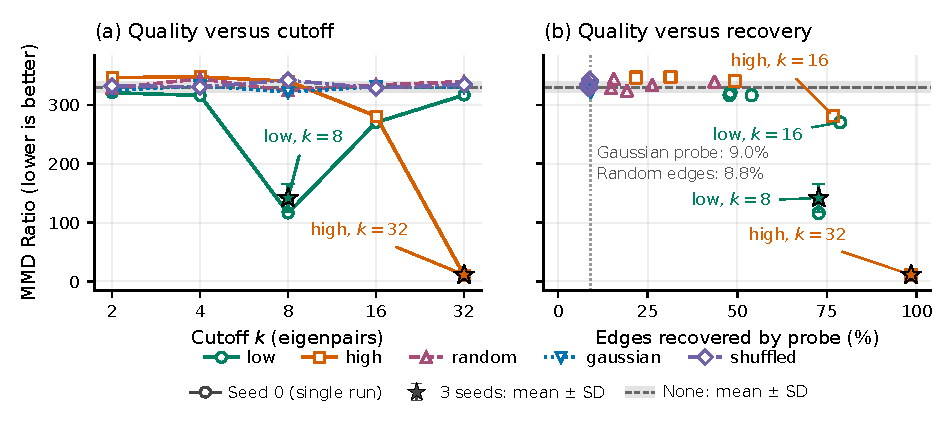
\includegraphics[width=\textwidth]{figures/sweep.pdf}
\caption{Oracle Planar sweep, five-metric validation Ratio. Hollow markers show seed 0;
stars show three-seed means and sample SD for repeated settings. The dashed baseline and gray
band show the unconditioned mean and SD, not significance. (a) Quality versus cutoff; lines
guide the eye. (b) Quality versus probe recovery.}
\label{fig:sweep}
\end{figure*}

More eigenpairs do not always help (Figure~\ref{fig:sweep}). In seed 0, low $k{=}8$ scores
116.3 and high $k{=}32$ scores 10.5, versus 335.7 for none. Other scores range from 270.5
to 347.9; smaller gains have not been repeated. Gaussian ranges from 322.1 to 332.5 and
shuffled from 328.8 to 342.0. These ranges do not measure baseline variation across seeds.

\begin{table}[t]
\centering\small
\setlength{\tabcolsep}{4pt}
\begin{tabular}{lccc}
\toprule
arm & Ratio $\downarrow$ & base/arm & valid \\
\midrule
\texttt{none} & 330.1 $\pm$ 7.5 & --- & 0\% \\
\texttt{low}, $k{=}8$ & 141.9 $\pm$ 23.6 & 2.3 & 0\% \\
\texttt{high}, $k{=}32$ & \textbf{11.1 $\pm$ 0.7} & 29.7 & 4.2\% \\
\bottomrule
\end{tabular}
\caption{Repeated settings: three-seed mean $\pm$ sample SD, five-metric validation Ratio.
Seed 0 also appears in the sweep. This is a separate set of runs from Table~\ref{tab:k8}:
low-$k{=}8$ averages 141.9 here and 158.0 there. High has 1/32, 2/32 and 1/32 valid samples
across seeds.}
\label{tab:spikes}
\end{table}

Seeds 1 and 2 confirm gains, not optimal cutoffs.

\subsection{How much of the target can be recovered?}
\label{sec:leakage}
\begin{table}[t]
\centering\small
\setlength{\tabcolsep}{4pt}
\begin{tabular}{lrrrrr}
\toprule
band & $k{=}2$ & $4$ & $8$ & $16$ & $32$ \\
\midrule
\texttt{low} & 48.1 & 54.0 & \textbf{72.7} & 78.7 & 47.9 \\
\texttt{high} & 21.8 & 31.4 & 49.3 & 76.7 & \textbf{98.5} \\
\texttt{random} & 14.8 & 15.6 & 19.2 & 26.3 & 43.6 \\
\texttt{gaussian} & 9.2 & 8.5 & 9.2 & 8.7 & 9.4 \\
\texttt{shuffled} & 8.7 & 8.7 & 8.8 & 8.7 & 8.3 \\
\bottomrule
\end{tabular}
\caption{Edges recovered by the privileged probe (\%) on Planar validation graphs. Bold marks
the selected generation settings. Random-edge chance is 8.8\%; Gaussian controls also account
for choosing the better score orientation.}
\label{tab:leakage}
\end{table}

Both selected conditions reveal many target edges (Table~\ref{tab:leakage}). At $k{=}8$,
low has both the best generation score and the highest recovery. High $k{=}32$ allows
98.5\% recovery, nearly reconstructing the target from its condition alone.

\paragraph{Reading the two axes.} Low-$k{=}8$ and high-$k{=}16$ have similar recovery
(72.7\% and 76.7\%) but different seed-0 Ratios (116.3 and 281.2) in Figure~\ref{fig:sweep}(b).
At $k{=}16$, low and high have both similar recovery (78.7\% and 76.7\%) and similar Ratios
(270.5 and 281.2). These are single-seed scores, not the low-$k{=}8$ three-seed mean of
141.9; neither $k{=}16$ setting was repeated. Recovery alone therefore does not consistently
rank quality. Still, similar scores from one probe do not mean the inputs contain equal
information. The first pair also differs in $k$ and graph-level input width. High-$k{=}32$
shows how much the hint reveals; probe recovery does not measure copying by the generator.

Low recovery falls to 47.9\% at $k{=}32$, while high recovery increases. A model need not
use all the information that the probe can recover. On SBM, low recovery rises from 33.8\%
to 74.4\% and high from 23.0\% to 87.7\%, above 9.4\% chance. This supports the recovery
finding on another dataset, not the generation finding.

\begin{figure*}[t]
\centering

\includegraphics[width=\textwidth]{figures/copying.pdf}
\caption{Validation graph 0 and low-$k{=}8$/unconditioned sample 0, seed 0. Panels share the
reference's node positions; this does not imply planarity. Solid green edges are shared; dashed
gray edges are not. Labels show shared/generated counts and $F_1$; Table~\ref{tab:copying}
covers all samples.}
\label{fig:copying}
\end{figure*}

\begin{table}[t]
\centering\small
\setlength{\tabcolsep}{4pt}
\begin{tabular}{lccc}
\toprule
band & matched $F_1$ & mismatched $F_1$ & top-1 \\
\midrule
\texttt{none} & .085 $\pm$ .004 & .085 & 2/96 \\
\texttt{low} & .617 $\pm$ .005 & .088 & 96/96 \\
\texttt{high} & .337 $\pm$ .005 & .087 & 96/96 \\
\texttt{random} & .108 $\pm$ .003 & .086 & 18/96 \\
\bottomrule
\end{tabular}
\caption{Copying check, 12 saved $k{=}8$ runs. Matched: source graph, three-seed mean $\pm$
sample SD; mismatched: other 31 graphs. Top-1 counts unique nearest matches; chance is 1/32.}
\label{tab:copying}
\end{table}

Using stored node order, we compare sample $i$ with source graph $i$. Low and high identify
their source uniquely in all 96 samples per band (Table~\ref{tab:copying}). None has almost
equal matched and mismatched overlap; random has a smaller gap than low or high.
Figure~\ref{fig:copying} shows one example.

The snapshot records source hashes; older analysis used different samples. Original MMD
reports lack sample hashes, preventing exact linkage. The copying analysis in
Table~\ref{tab:copying} covers 12 runs at $k{=}8$.

\subsection{Few generated graphs are valid}
\label{sec:validity}
All 384 saved $k{=}8$ samples are nonplanar, although 67.7\% of low and 91.7\% of
unconditioned samples are connected. High-$k{=}32$ repeat reports include 4/96 valid graphs.
Separately, its probe gives 1/32 planar graphs despite 98.5\% recovery. Near-complete edge
recovery does not guarantee planarity with this decoder; it does not follow that validity
requires exact copying or that the dataset causes the failures.

\subsection{Using more compute}
\label{sec:budget}
In a separate five-metric discrete model \citep{austin2021d3pm}, ten layers, 500 steps and
1,000 epochs improve unconditioned Ratio from 306.78 to 39.60. Conditioning reaches 15.40,
shrinking the gap from 276.7 to 24.2. Each setting has one validation run. Validity stays zero.
This is not a DiGress reproduction; gains over a small baseline need not stay the same at
a larger budget.

\subsection{Does augmentation help classification?}
\label{sec:downstream}
This secondary experiment asks whether generated graphs help a separate GNN predict SBM
community count (2--5). ``Real'' graphs come from the SBM recipe. Augmentation adds one diffusion sample per real
graph, using either no hint or high-$k{=}32$ hints. The three-layer dense Graph Isomorphism
Network (GIN), hidden width 64, trains on 20/40/80 real graphs with five seeds. Communities
have 20--40 nodes, $p_{\rm intra}=0.3$, $p_{\rm inter}=0.05$. We select models on 60 validation
graphs and evaluate on 100 separate test graphs.

\begin{table}[t]
\centering\small
\setlength{\tabcolsep}{4pt}
\begin{tabular}{rccc}
\toprule
\shortstack{Real training\\graphs} & Real only & + No hint & \shortstack{+ High\\$k{=}32$} \\
\midrule
20 & \textbf{94.8} & 89.8 & 92.0 \\
40 & \textbf{97.0} & 94.2 & 94.0 \\
80 & \textbf{97.2} & 96.2 & 95.0 \\
\bottomrule
\end{tabular}
\caption{Mean test accuracy (\%), five seeds; higher is better. The last two columns add
graphs from the unconditioned or high-frequency-conditioned generator. These are descriptive
means, not significance tests.}
\label{tab:downstream}
\end{table}

\textbf{Neither diffusion method improves average accuracy over real-only training}
(Table~\ref{tab:downstream}). High beats no hints at 20 real graphs, but not at 40 or 80.
Adding fresh SBM-recipe graphs instead reaches 98.8\% at 80 real graphs, versus 97.2\%
for real-only.

This is a limited negative result, not evidence against augmentation in general. Generated
graphs inherit template labels without checking their community count; label errors may hurt
accuracy, but we did not measure their effect. Graph size is also an easy clue: a CPU
nearest-class-mean classifier using only node count, fitted without tuning on the same
training sets, scores 82.2/82.8/82.6\% on the same test set. Unconditioned samples still
receive node count, so inherited labels need not be independent of them. Finally, we tested
high-$k{=}32$, not low-frequency augmentation, and did not check SBM samples for duplication.
The experiment does not tell us whether correctly labeled, low-frequency-generated graphs
would help.

\section{Discussion and Limitations}
\label{sec:discussion}
A strength of this study is combining generation scores with recovery and copying checks.
This helps distinguish improved statistics from reconstruction, although separating frequency
from target information still needs further controls.

Generation is evaluated on Planar validation graphs. Selected settings have three seeds;
most cutoffs have one. Generalization needs more seeds, datasets and untouched-test evaluation.
The sweep supports aggregate comparisons; detailed component metrics are available for the pilot.

Our snapshot makes copying checks reproducible for conditioning graphs in fixed node order,
not training graphs under arbitrary relabeling. Latent diffusion, cluster conditioning,
combinatorial Laplacians and SignNet offer further comparisons. SBM results cover low- and
high-band recovery, not a generation sweep; its shuffled control is excluded because graph
sizes are not matched.

\begin{samepage}
\section{Conclusion}
We studied spectral hints in graph diffusion and found repeatable improvements at low
$k{=}8$ and high $k{=}32$ under oracle conditioning on Planar. Our main contribution is to
pair generation scores with direct measurements of target recovery and source-graph
similarity. These checks show why improvements should be read alongside reconstruction,
rather than attributed to frequency alone. The code and sample snapshot make the copying
analysis reusable. Together, the results and evaluation tools provide a practical starting
point for testing spectral guidance across other graph families and model designs.
\par
\end{samepage}

\clearpage
\bibliography{custom}

\end{document}
